\documentclass[a6paper,landscape,10pt]{report}

\usepackage[utf8]{inputenc}
\usepackage[portuguese]{babel}
\usepackage[top=1cm,left=.2cm,right=.4cm,bottom=.8cm,footskip=0cm]{geometry} %Define margens e distância do rodapé
\usepackage{titletoc} %Para definir o estilo da lista de conteúdo
\usepackage[toc]{multitoc} %Para lista de conteúdo com 3 colunas
\usepackage{pdfpages} %Para incluir pdfs
\usepackage{fancyhdr} %Para personalizar cabeçalho e rodapé
\usepackage[none]{hyphenat} %Impedir quebra de palavras no fim da linha
% \usepackage[sfdefault,condensed]{cabin}
% \usepackage[T1]{fontenc}
%\usepackage[sfdefault]{roboto}  %% Option 'sfdefault' only if the base font of the document is to be sans serif
%\usepackage[T1]{fontenc}
\usepackage{anyfontsize}

\usepackage{PTSansNarrow}
\renewcommand*\familydefault{\sfdefault} %% Only if the base font of the document is to be sans serif
\usepackage[T1]{fontenc}

% \usepackage[scaled]{helvet}
% \renewcommand*\familydefault{\sfdefault} %% Only if the base font of the document is to be sans serif
% \usepackage[T1]{fontenc}

%\renewcommand*\rmdefault{pag}

\pdfminorversion=5
\pdfcompresslevel=9
\pdfobjcompresslevel=2


%Define novo estilo de cabeçalho e rodapé
\fancypagestyle{plain}{%
  \renewcommand{\headrulewidth}{0pt}%Sem linha de cabeçalho
  \fancyfoot[C]{} %Sem nada no centro do rodapé
  \fancyfoot[R]{\fontfamily{phv}\selectfont\Large\textbf{\thepage}} %Número da página grande e em negrito à direita do rodapé
}

\renewcommand*{\multicolumntoc}{3} %Define 3 colunas para a lista de conteúdo

\newcommand{\capa}[1]{\includepdf[pagecommand={\thispagestyle{empty}}]{../capas/#1.pdf}}

%Define estilo dos capítulos no índice
\titlecontents{chapter}
[.3cm] %espaço à esquerda
{\addvspace{.8em}\bf\contentsmargin{0em}} %formatação do título e espaço vertical antes
{} %formato de número
{} %formato de número sem título
{\vspace*{.4em}} %filler
[] %espaço depois do título

%Define estilo da seção no índice
\titlecontents{section}
[.2cm] %espaço à esquerda
{\small} %formatação do título e espaço vertical antes
{} %formato de número
{\textbf{\contentspage}\hspace{2em}} %formato de número sem título
{\hfill} %filler
[] %espaço depois do título

% \makeatletter
% \def\l@chapter#1#2{%
% \pagebreak[3]
% \vskip .75em plus 1pt \@tempdima 1em
% \begingroup
%   \parindent \z@ \rightskip \@pnumwidth
%   \parfillskip -\@pnumwidth
%   \advance\leftskip\@tempdima
%   \hskip 0em
%   \leavevmode \bfseries \MakeUppercase{#1}
%   \par
% \endgroup
% }
% \makeatother

\begin{document}

%Sem numeração nas primeiras páginas
\pagestyle{empty}

\capa{capa}

%Cria lista de conteúdo sem cabeçalho
\begingroup
\makeatletter
\@starttoc{toc}
\makeatother
\endgroup

%Define estilo das páginas incluídas como PDF
\includepdfset{pagecommand={\thispagestyle{plain}}}

%Começa o livro
\newpage
\addcontentsline{toc}{chapter}{RANCHOS} %Inclui novo capítulo no índice
\capa{rancho}
\addcontentsline{toc}{section}{A Praça} %Inclui nova partitura no índice
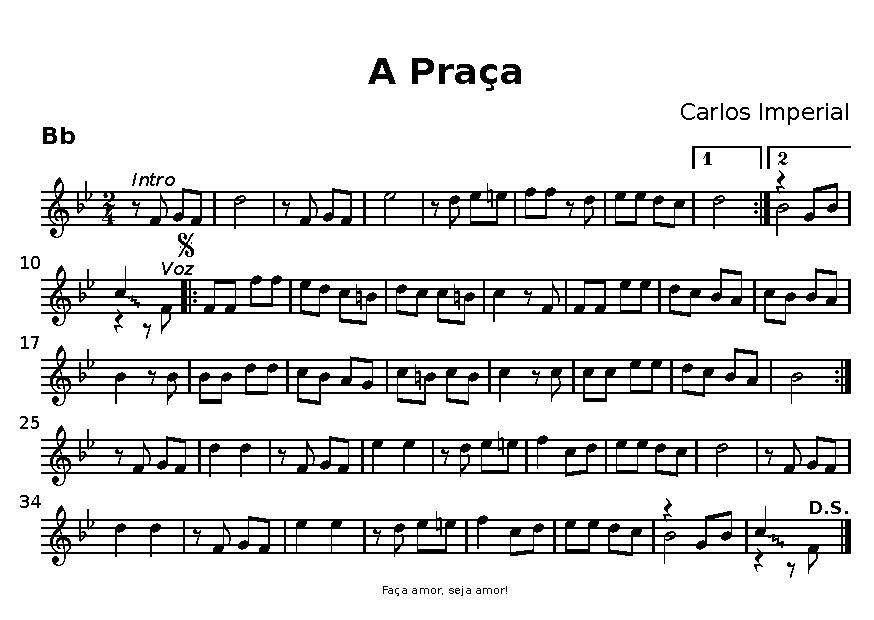
\includepdf{../PDF/aPraca.pdf}
\addcontentsline{toc}{section}{As Pastorinhas}
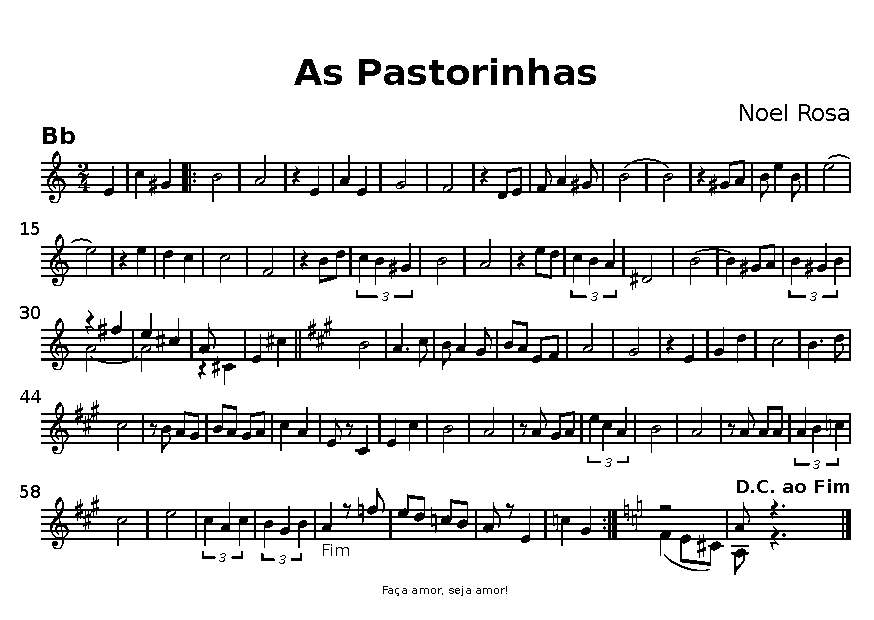
\includepdf{../PDF/pastorinhas.pdf} %Inclui a partitura no songbook
%\addcontentsline{toc}{section}{Até quarta-feira}
%\addcontentsline{toc}{section}{Avenida Iluminada}
%\addcontentsline{toc}{section}{Baile no Municipal}
\addcontentsline{toc}{section}{Bandeira Branca}
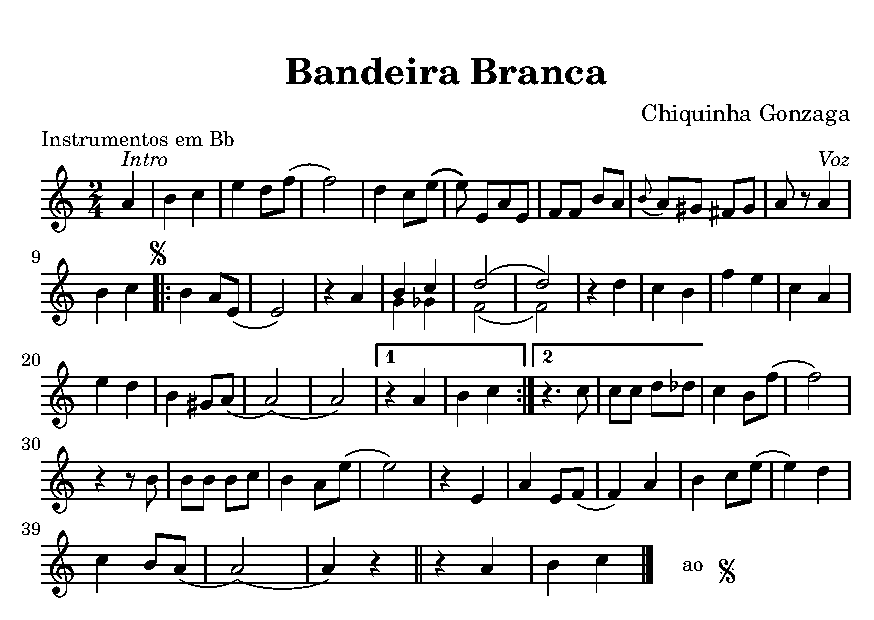
\includepdf{../PDF/bandeiraBranca.pdf}
\addcontentsline{toc}{section}{Carinhoso}
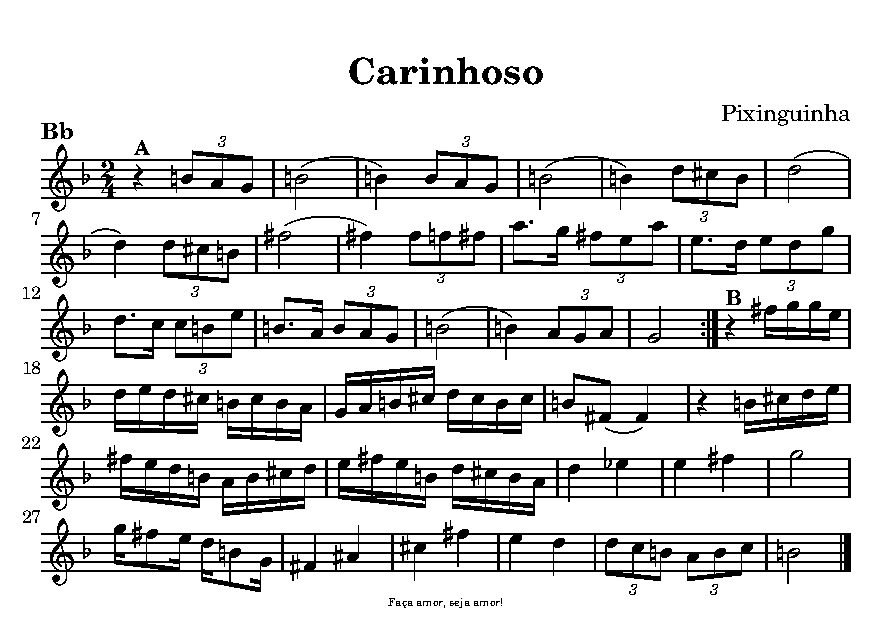
\includepdf{../PDF/carinhoso.pdf}
%\addcontentsline{toc}{section}{Estrela do Mar}
%\addcontentsline{toc}{section}{Eu quero é botar...}
%\addcontentsline{toc}{section}{Máscara Negra}
%\addcontentsline{toc}{section}{Noite dos mascarados}
\addcontentsline{toc}{section}{Ô Abre Alas}
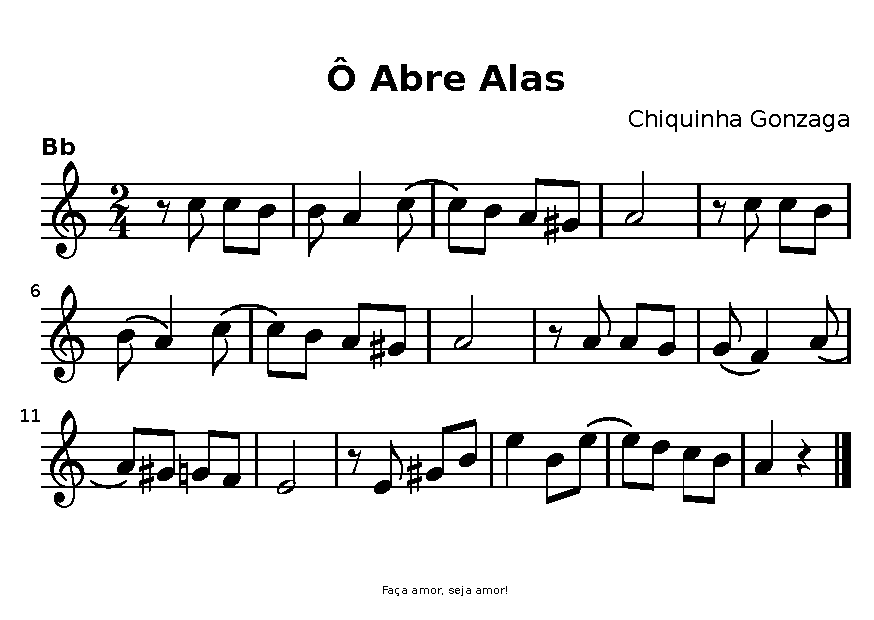
\includepdf{../PDF/abreAlas.pdf}

\addcontentsline{toc}{chapter}{CRÁSSICAS}
\capa{crassicas}
% \addcontentsline{toc}{section}{A patroa me contou...}
\addcontentsline{toc}{section}{Allah-La Ô}
\includepdf{../PDF/allahlao.pdf}
\addcontentsline{toc}{section}{Aurora}
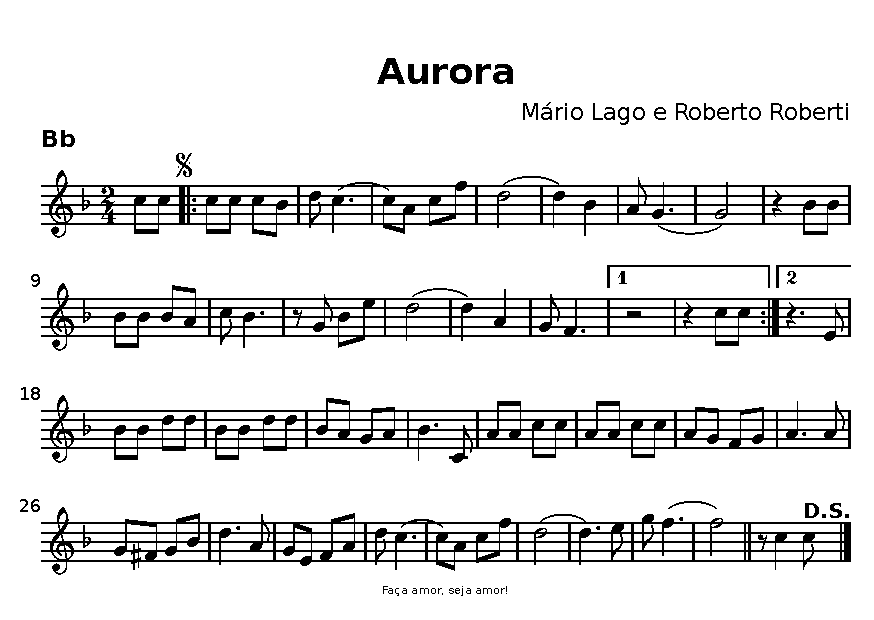
\includepdf{../PDF/aurora.pdf}
% \addcontentsline{toc}{section}{Balança o saco}
 \addcontentsline{toc}{section}{Balancê}
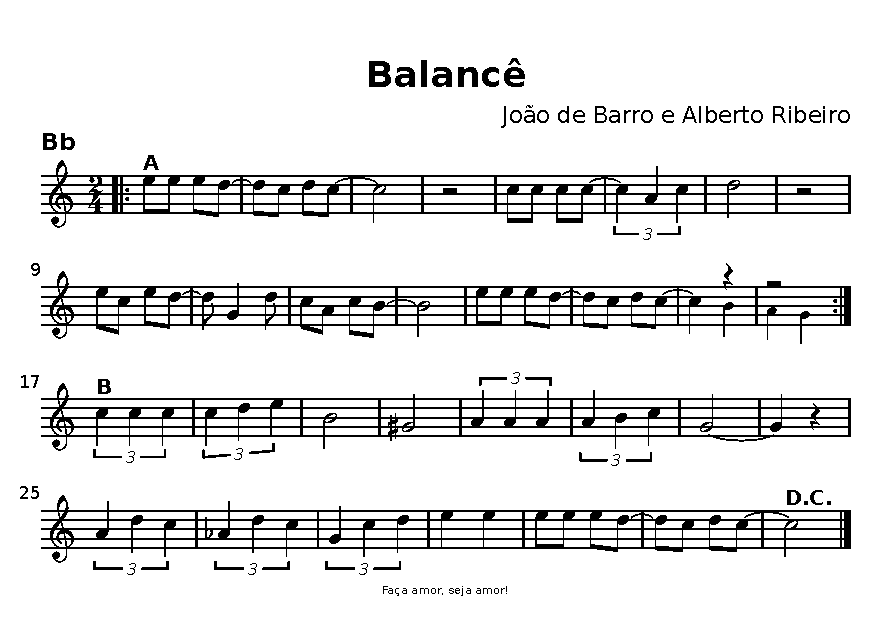
\includepdf{../PDF/balance.pdf}
% \addcontentsline{toc}{section}{Bota a Camisinha}
\addcontentsline{toc}{section}{Cabeleira do Zezé}
\includepdf{../PDF/cabeleiraDoZeze.pdf}
\addcontentsline{toc}{section}{Cachaça}
\includepdf{../PDF/cachaca.pdf}
% \addcontentsline{toc}{section}{Caiu na rede é peixe}
% \addcontentsline{toc}{section}{Can Can no Carnaval}
\addcontentsline{toc}{section}{Chiquita Bacana}
\includepdf{../PDF/chiquitaBacana.pdf}
% \addcontentsline{toc}{section}{Cidade Maravilhosa}
\addcontentsline{toc}{section}{Coração de Jacaré}
\includepdf{../PDF/coracaoDeJacare.pdf}
% \addcontentsline{toc}{section}{Daqui não saio}
% \addcontentsline{toc}{section}{Está chegando a hora}
\addcontentsline{toc}{section}{Índio quer apito}
\includepdf{../PDF/indio.pdf}
\addcontentsline{toc}{section}{A Jardineira}
\includepdf{../PDF/jardineira.pdf}
% \addcontentsline{toc}{section}{Mamãe eu quero}
\addcontentsline{toc}{section}{Marcha da Cueca}
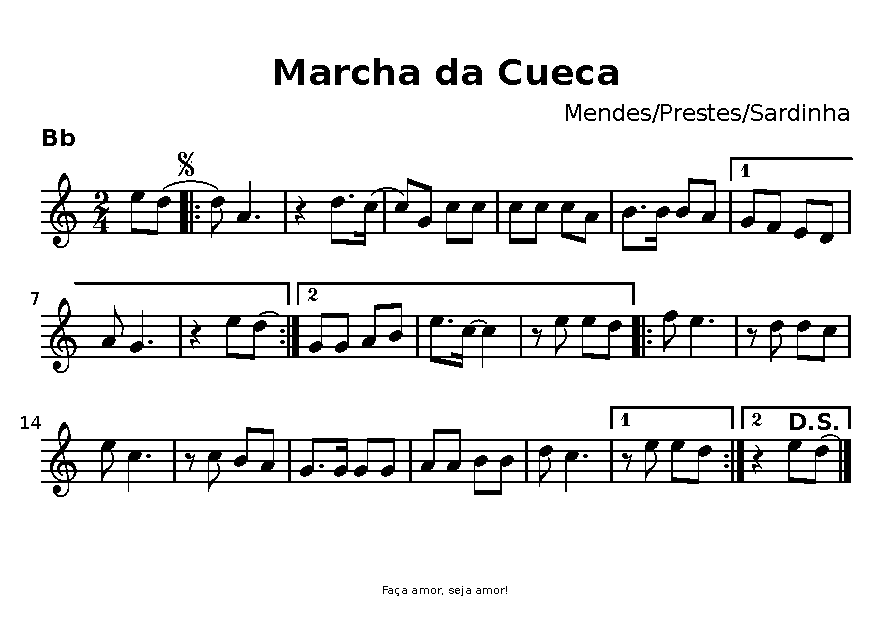
\includepdf{../PDF/marchaDaCueca.pdf}
% \addcontentsline{toc}{section}{Marcha do Cordão...}
\addcontentsline{toc}{section}{Marcha do Remador}
\includepdf{../PDF/remador.pdf}
% \addcontentsline{toc}{section}{Maria Sapatão}
% \addcontentsline{toc}{section}{Me dá um dinheiro aí}
% \addcontentsline{toc}{section}{Mulata iê iê iê}
% \addcontentsline{toc}{section}{Pegando Fogo}
% \addcontentsline{toc}{section}{Pescador}
% \addcontentsline{toc}{section}{Pierrô Apaixonado}
% \addcontentsline{toc}{section}{Quem sabe sabe}
% \addcontentsline{toc}{section}{Ressaca}
% \addcontentsline{toc}{section}{Saca-Rolha}
% \addcontentsline{toc}{section}{Sassaricando}
% \addcontentsline{toc}{section}{Taí}
% \addcontentsline{toc}{section}{Tem nêgo bêbo aí}
% \addcontentsline{toc}{section}{Tomara que chova}
% \addcontentsline{toc}{section}{Turma do Funil}
% \addcontentsline{toc}{section}{Vai com jeito}
% \addcontentsline{toc}{section}{Zé Pereira}

\addcontentsline{toc}{chapter}{BELLOT}
\capa{bellot}
\addcontentsline{toc}{section}{Jingle Tarifa Zero}
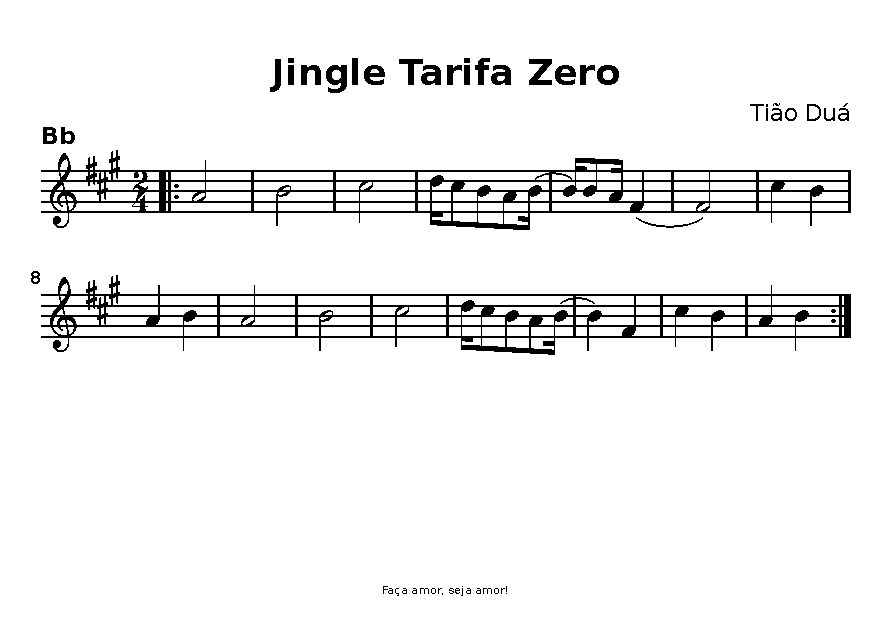
\includepdf{../PDF/jingleTarifaZero.pdf}
\addcontentsline{toc}{section}{Mambo da Gameleira}
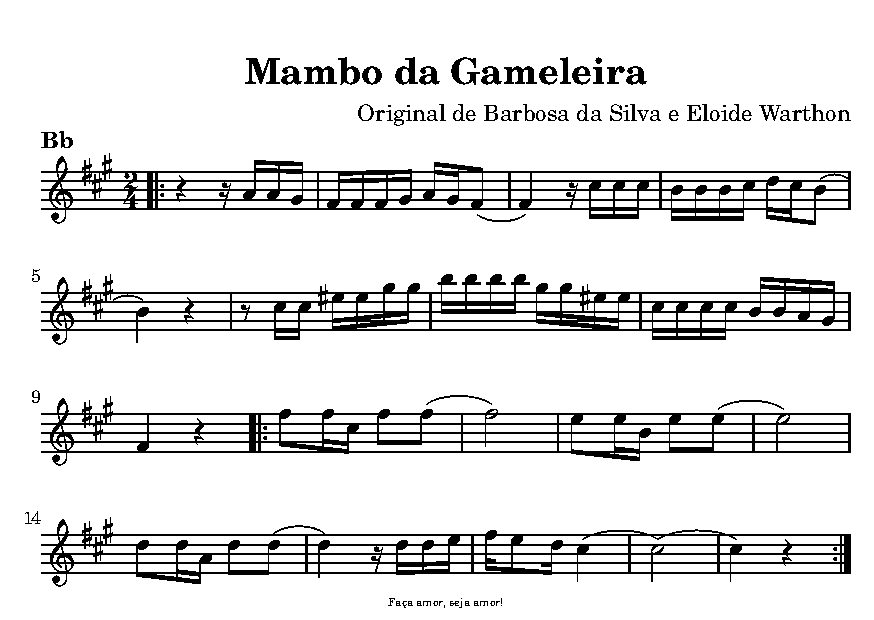
\includepdf{../PDF/mamboGameleira.pdf}
%\addcontentsline{toc}{section}{Pula Catraca\\Bibi Fomfom}
%\addcontentsline{toc}{section}{Coxinha da Madrasta}
%\addcontentsline{toc}{section}{Então Brilha}
%\addcontentsline{toc}{section}{Filhos de Chachá}
\addcontentsline{toc}{section}{Mamá na Vaca}
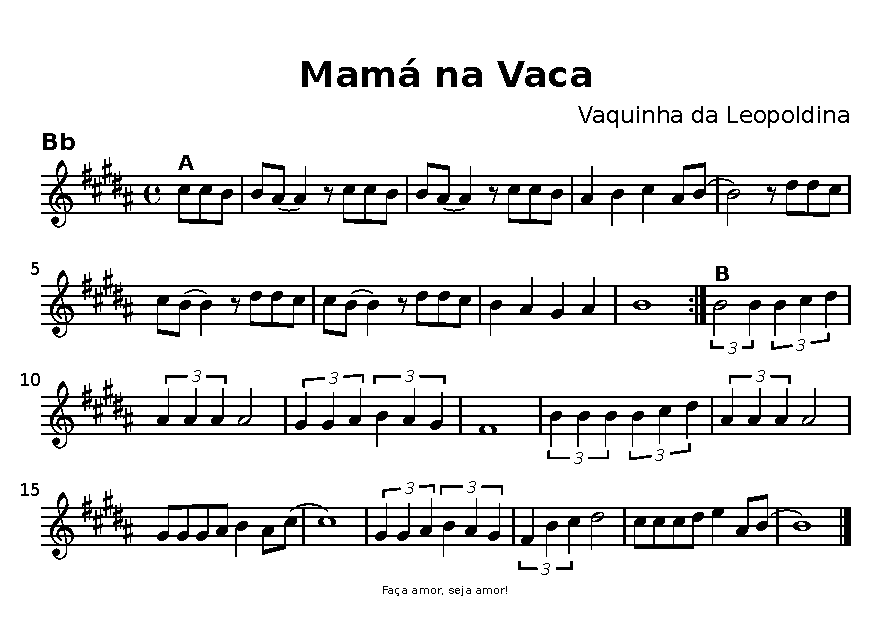
\includepdf{../PDF/mamaNaVaca.pdf}
%\addcontentsline{toc}{section}{Marcha da Alcova}
\addcontentsline{toc}{section}{Marcha da Praia}
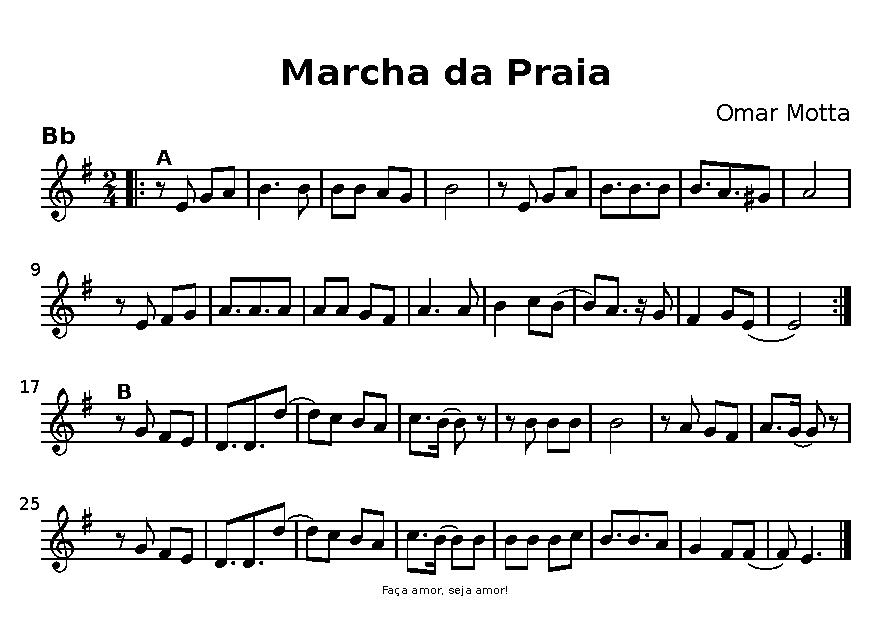
\includepdf{../PDF/praia.pdf} %Inclui a partitura no songbook
\addcontentsline{toc}{section}{Marcha do Manjericão}
\includepdf{../PDF/manjericao.pdf}
%\addcontentsline{toc}{section}{O Baile do Pó Royal}

\addcontentsline{toc}{chapter}{AXÉ}
\capa{axe}
%\addcontentsline{toc}{section}{A dança do bum bum}
\addcontentsline{toc}{section}{A Luz de Tieta}
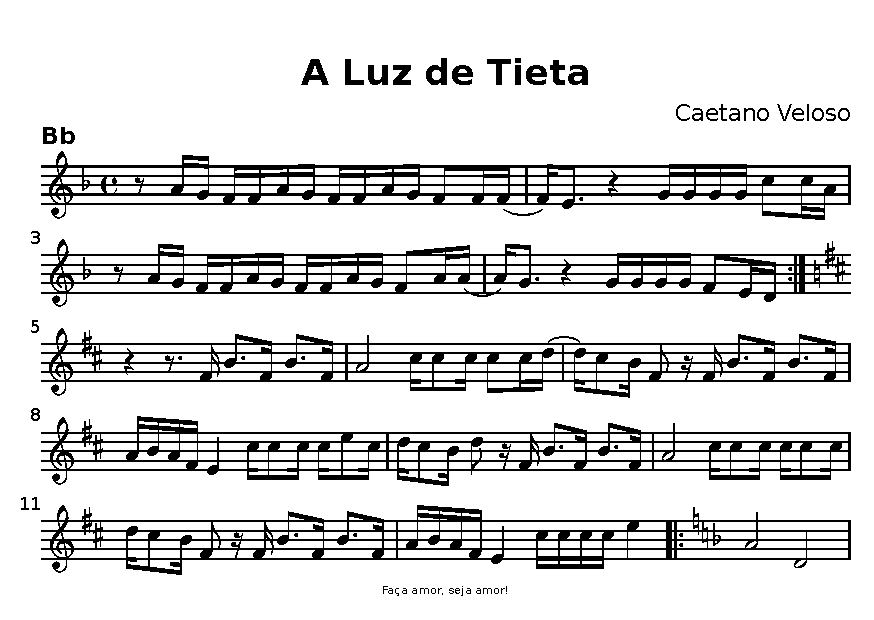
\includepdf{../PDF/luzTieta.pdf}
%\addcontentsline{toc}{section}{Água Mineral}
%\addcontentsline{toc}{section}{Alô Paixão}
%\addcontentsline{toc}{section}{Baianidade Nagô}
%\addcontentsline{toc}{section}{Beija-Flor}
%\addcontentsline{toc}{section}{Beleza Rara}
%\addcontentsline{toc}{section}{Berimbau Metalizado}
%\addcontentsline{toc}{section}{Boquinha da garrafa}
%\addcontentsline{toc}{section}{Céu da boca}
%\addcontentsline{toc}{section}{Cordeiro de Nanã}
%\addcontentsline{toc}{section}{De Ladinho}
%\addcontentsline{toc}{section}{Eu também quero beijar}
%\addcontentsline{toc}{section}{Libera Geral}
%\addcontentsline{toc}{section}{Me abraça, me beija}
%\addcontentsline{toc}{section}{Mila}
%\addcontentsline{toc}{section}{Nossa gente (Avisa lá)}
%\addcontentsline{toc}{section}{O canto da cidade}
%\addcontentsline{toc}{section}{Prefixo do Verão}
%\addcontentsline{toc}{section}{Rapunzel}
%\addcontentsline{toc}{section}{Requebra }
%\addcontentsline{toc}{section}{Sexy Iemanjá}

%\addcontentsline{toc}{chapter}{A LAMBÁSTICA \\ARROCHERIA \\FORROBÓTICA \\FREVALÍSTICA}
\addcontentsline{toc}{chapter}{A LAMBÁSTICA ARROCHERIA \\FORROBÓTICA FREVALÍSTICA}
\capa{lambastica}
%\addcontentsline{toc}{section}{Anunciação}
%\addcontentsline{toc}{section}{La belle du jour}
%\addcontentsline{toc}{section}{Girassol}
%\addcontentsline{toc}{section}{Morena Tropicana}
%\addcontentsline{toc}{section}{Acorda Maria Bonita}
%\addcontentsline{toc}{section}{Que nem Jiló}
%\addcontentsline{toc}{section}{Fui Fiel}
%\addcontentsline{toc}{section}{Porque Homem não chora}
%\addcontentsline{toc}{section}{Chorando se Foi}
%\addcontentsline{toc}{section}{Haja Amor}
%\addcontentsline{toc}{section}{Lindo Lago do Amor}
%\addcontentsline{toc}{section}{Atras do trio elétrico}
%\addcontentsline{toc}{section}{Banho de cheiro}
%\addcontentsline{toc}{section}{Bloco do Prazer}
%\addcontentsline{toc}{section}{Não existe pecado ao...}
%\addcontentsline{toc}{section}{Um frevo novo}
%\addcontentsline{toc}{section}{Vassourinhas}

\addcontentsline{toc}{chapter}{SAMBENHAS E PRIMOS TORTOS}
\capa{samba}
%\addcontentsline{toc}{section}{Saudades da Amélia}
%\addcontentsline{toc}{section}{Cilada}
%\addcontentsline{toc}{section}{Ê baiana}
%\addcontentsline{toc}{section}{Kid Cavaquinho}
%\addcontentsline{toc}{section}{Recordar é viver}
%\addcontentsline{toc}{section}{Trem das Onze}
%\addcontentsline{toc}{section}{Tristeza}
%\addcontentsline{toc}{section}{Maracangalha}

\addcontentsline{toc}{chapter}{FUNK}
\capa{funk}
%\addcontentsline{toc}{section}{Beijinho no ombro}
%\addcontentsline{toc}{section}{Dom Dom Dom}
%\addcontentsline{toc}{section}{Glamurosa}
%\addcontentsline{toc}{section}{Morto muito louco}
%\addcontentsline{toc}{section}{Rap da Felicidade}
%\addcontentsline{toc}{section}{Rap das Armas}
%\addcontentsline{toc}{section}{Show das poderosas}

\addcontentsline{toc}{chapter}{AFRODITE SE QUISER}
\capa{afrodite}
\addcontentsline{toc}{section}{Besame Mucho}
\includepdf{../PDF/besame.pdf}
%\addcontentsline{toc}{section}{Emoções}
%\addcontentsline{toc}{section}{Quizas}
%\addcontentsline{toc}{section}{Garçon}

\addcontentsline{toc}{chapter}{SLOW MOTION}
\capa{slow}
\addcontentsline{toc}{section}{Assim falou zaratrusta}
\includepdf{../PDF/odisseia.pdf}
\addcontentsline{toc}{section}{Carroça de Fogo}
\includepdf{../PDF/carroca.pdf}

\addcontentsline{toc}{chapter}{CHAMA O SÍNDICO}
\capa{sindico}
%\addcontentsline{toc}{section}{Acenda o farol}
%\addcontentsline{toc}{section}{Azul da cor do mar}
%\addcontentsline{toc}{section}{Batata frita}
%\addcontentsline{toc}{section}{Bom senso}
%\addcontentsline{toc}{section}{Canário do Reino}
%\addcontentsline{toc}{section}{Chove Chuva}
%\addcontentsline{toc}{section}{Contato com o Mundo\\Flores Belas}
%\addcontentsline{toc}{section}{Cristina}
%\addcontentsline{toc}{section}{Ela partiu}
%\addcontentsline{toc}{section}{Fio Maravilha}
%\addcontentsline{toc}{section}{Gostava tanto de você}
%\addcontentsline{toc}{section}{Guiné Bissau...}
%\addcontentsline{toc}{section}{Imunização Racional...}
%\addcontentsline{toc}{section}{Ive Brussel}
%\addcontentsline{toc}{section}{Márcio Leonardo e Telmo}
%\addcontentsline{toc}{section}{Menina mulher}
%\addcontentsline{toc}{section}{Meus Filhos\\Que beleza}
%\addcontentsline{toc}{section}{Não quero dinheiro}
\addcontentsline{toc}{section}{País Tropical}
\includepdf{../PDF/paTroPi.pdf}
%\addcontentsline{toc}{section}{Primavera}
%\addcontentsline{toc}{section}{Quem cochicha...}
%\addcontentsline{toc}{section}{Sossego}
%\addcontentsline{toc}{section}{Taj Mahal}
%\addcontentsline{toc}{section}{Terapêutica do grito}
%\addcontentsline{toc}{section}{Umbabarauma}
%\addcontentsline{toc}{section}{W Brasil}
%\addcontentsline{toc}{section}{Zumbi}

\addcontentsline{toc}{chapter}{OUTRAS}
\capa{outras}
\addcontentsline{toc}{section}{A barata diz que tem}
\includepdf{../PDF/barata.pdf}
%\addcontentsline{toc}{section}{Cant buy me love}
%\addcontentsline{toc}{section}{I wanna hold your hand}
%\addcontentsline{toc}{section}{Lua de cristal}
%\addcontentsline{toc}{section}{Pedro de Lara}
%\addcontentsline{toc}{section}{Superfantástico}
%\addcontentsline{toc}{section}{Uma brasileira}
%\addcontentsline{toc}{section}{Aflorou}

\end{document}
